\def \course {برنامه ریزی خطی}
\def \titlename {تمرین‌های تحویلی فصل ۱}
\def \name {ابراهیم نجاتی}
\def \studentnumber{۹۸۰۰۰۰۰۰۰۰}

%%% Local Variables:
%%% coding: utf-8
%%% mode: latex
%%% TeX-engine: xetex
%%% End:

% Hardcode the templates directiry
\documentclass[a4paper,12pt]{article}

% Strech line distances
% \renewcommand{\baselinestretch}{1.3}
\usepackage{amsmath}
\pagestyle{plain}
\usepackage{graphicx}

\usepackage{hyperref}
\hypersetup{
    colorlinks=true,
    linkcolor=blue,
    filecolor=magenta,
    urlcolor=blue,
  }

% Margins act weird with headers
\usepackage[
    %margin=1.5cm,
    %includehead,includefoot,
    hmargin=1.5cm,
    top=2.5cm
    ]{geometry}

\usepackage{fancyhdr}

% reach maximum nesting
\usepackage{enumitem}
\usepackage{longtable}

% Show source code
\usepackage{listings}
\usepackage{xcolor}

\definecolor{codegreen}{rgb}{0,0.6,0}
\definecolor{codegray}{rgb}{0.5,0.5,0.5}
\definecolor{codepurple}{rgb}{0.58,0,0.82}
\definecolor{backcolour}{rgb}{0.95,0.95,0.92}

\lstdefinestyle{mystyle}{
    backgroundcolor=\color{backcolour},
    commentstyle=\color{codegreen},
    keywordstyle=\color{magenta},
    numberstyle=\tiny\color{codegray},
    stringstyle=\color{codepurple},
    basicstyle=\ttfamily\footnotesize,
    breakatwhitespace=false,
    breaklines=true,
    captionpos=b,
    keepspaces=true,
    numbers=left,
    numbersep=5pt,
    showspaces=false,
    showstringspaces=false,
    showtabs=false,
    tabsize=2
}

\lstset{style=mystyle}

% Plots
\usepackage{pgfplots}
\usepgfplotslibrary{fillbetween}

\usepackage[localise=on]{xepersian}
\settextfont{XBZar}[
  Path = ./template/Zar/,
  UprightFont = *-Regular,
  BoldFont = *-Bold,
  ItalicFont = *-Italic,
  BoldItalicFont = *-BoldItalic,
  Extension = .ttf,
] % Fancy fonts, eh?

% Hmmm
\ExplSyntaxOn
\cs_set_eq:NN
\etex_iffontchar:D
\tex_iffontchar:D
\cs_undefine:N \c_one
\int_const:Nn \c_one { 1 }
\ExplSyntaxOff
\setmathdigitfont{XBZar}[
  Path = ./template/Zar/,
  UprightFont = *-Regular,
  BoldFont = *-Bold,
  ItalicFont = *-Italic,
  BoldItalicFont = *-BoldItalic,
  Extension = .ttf,
]
\setdigitfont{XBZar}[
  Path = ./template/Zar/,
  UprightFont = *-Regular,
  BoldFont = *-Bold,
  ItalicFont = *-Italic,
  BoldItalicFont = *-BoldItalic,
  Extension = .ttf,
]

% Change the formatting of `sections`
%\usepackage{sectsty}
%\allsectionsfont{\settextfont{Sahel}}

\fancypagestyle{firststyle} {
  \rhead{\course \\

     نام و نام خانوادگی: \name \\
    شماره دانشجویی: \studentnumber
    % آدرس ایمیل: ‌\email
  }

  \chead{\textbf{\Large \titlename} \\}
  \lhead{
\includegraphics[
    height=1.3cm]{./template/ferdowsi-logo.png} \\ \today}
  \headsep 5.5em
}
% Put style only on first page
\thispagestyle{firststyle}


\begin{document}

\section*{پاسخ به سؤالات}
\subsection*{سؤال ۹}
برای حلّ مسئله، تابع هدف را مینیمم‌سازی هزینه تولید درنظر می‌گیریم که در آن $x_{i}$ ساعت کار ماشین $i$ در یک هفته است.
\begin{align*}
  \text{min} \quad
  30x_{A} + 50x_{B} + 80x_{C}&
\end{align*}
اکنون با توجه به مقدار تیرآهن مورد نیاز، بقیه گذاره‌ها را نیز کامل می‌کنیم. همچنین می‌دانیم ساعت کار هر دستگاه در هفته محدود است.
\begin{align*}
  \text{min} \quad
  &30x_{A} + 50x_{B} + 80x_{C} \\
  \text{s.t.} \quad
  &350x_{A} + 650x_{B} + 850x_{C} = 12000 \\
  &250x_{A} + 400x_{B} + 700x_{C} = 6000 \\
  &200x_{A} + 350x_{B} + 600x_{C} = 5000 \\
  &125x_{A} + 200x_{B} + 325x_{C} = 7000 \\
  &0 \leq x_{i} \leq 50 \quad
  i \in \{A, B, C\} \\
\end{align*}

\subsection*{سؤال ۱۰}
برای حلّ مسئله، تابع هدف را مینیمم‌سازی هزینه نفت خام است که در آن $x_{1}$ تعداد بشکه‌های نفت خام سبک و $x_{2}$ تعداد بشکه‌های نفت خام سنگین است.
\begin{align*}
  \text{min} \quad
  &20x_{1} + 15x_{2} \\
  \text{s.t.} \quad
  &0.4x_{1} + 0.32x_{2} = 10^{6} \\
  &0.2x_{1} + 0.4x_{2} = 5 \times 10^{5} \\
  &0.35x_{1} + 0.2x_{2} = 3 \times 10^{5} \\
  &x_{i} \geq 0 \quad
  i \in \{1, 2\} \\
\end{align*}

\subsection*{سؤال ۱۴}
برای حلّ مسئله، تابع هدف را مینیمم‌سازی هزینه حمل و نقل می‌گیریم که در آن $x_{ij}$ مقدار تخته‌ای است از شرکت تخته‌سازی $i$ام به کارخانه مبل $j$ام باید منتقل شود.
\begin{align*}
  \text{min} \quad
  x_{11} + 3x_{12} + 5x_{13} +
  3.5x_{21} + 4x_{22} + 4.8x_{23} +
  3.5x_{31} + 3.6x_{32} + 3.2x_{33}
\end{align*}
احتیاج کارخانه‌های مبل به صورت زیر است.
\begin{align*}
  x_{11} + x_{21} + x_{31} &= 500 \\
  x_{12} + x_{22} + x_{32} &= 700 \\
  x_{13} + x_{23} + x_{33} &= 600 \\
\end{align*}
محدودیت کارخانه تخته‌سازی سوم در ساخت و محدودیت کارخانه‌های تخته‌سازی اول و دوم در حمل و نقل نیز به صورت زیر است:
\begin{align*}
  &x_{31} + x_{32} + x_{33} \leq 500 \\
  &0 \leq x_{1j} \quad j \in \{1, 2, 3\} \\
  &0 \leq x_{ij} \leq 200 \quad
  i \in \{1, 2\} \land j \in \{1, 2, 3\}
\end{align*}
پس در نهایت داریم:
\begin{align*}
  \text{min} \quad
  &x_{11} + 3x_{12} + 5x_{13} +
  3.5x_{21} + 4x_{22} + 4.8x_{23} +
  3.5x_{31} + 3.6x_{32} + 3.2x_{33} \\
  \text{s.t.} \quad
  &x_{11} + x_{21} + x_{31} = 500 \\
  &x_{12} + x_{22} + x_{32} = 700 \\
  &x_{13} + x_{23} + x_{33} = 600 \\
  &x_{31} + x_{32} + x_{33} \leq 500 \\
  &0 \leq x_{1j} \quad j \in \{1, 2, 3\} \\
  &0 \leq x_{ij} \leq 200 \quad
  i \in \{1, 2\} \land j \in \{1, 2, 3\}
\end{align*}

\subsection*{سؤال ۳۰}
ابتدا با توجه به علامت هر متغیر، جایگزین آن‌را قرار می‌دهیم:
\begin{align*}
  &x_{1} = x^{+}_{1} - x^{-}_{1}
  &&x_{2} = x^{+}_{2} - x^{-}_{2}
  &&x_{3} = - 3 - \bar{x_{3}} \\
  &x^{+}_{1} , x^{-}_{1} \geq 0
  &&x^{+}_{2} , x^{-}_{2} \geq 0
  &&\bar{x_{3}} = -3 -x_{3}
\end{align*}
الف) پس مسأله را به صورت زیر بازنویسی می‌کنیم:
\begin{alignat*}{7}
  &\text{min} \quad&
  (x^{+}_{1} - x^{-}_{1})
  -&&(x^{+}_{2} - x^{+}_{2})
  -&&3(-3 -\bar{x_{3}})\\
  &\text{s.t.} \quad&
  -(x^{+}_{1} - x^{-}_{1})
  +&&3(x^{+}_{2} - x^{+}_{2})
  +&&(-3 -\bar{x_{3}})
  &-s_{1} = 13 \\
  &&(x^{+}_{1} - x^{-}_{1})
  +&&2(x^{+}_{2} - x^{+}_{2})
  +&&3(-3 -\bar{x_{3}})
  &+s_{1} = 12 \\
  &&2(x^{+}_{1} - x^{-}_{1})
  -&&(x^{+}_{2} - x^{+}_{2})
  +&&(-3 -\bar{x_{3}}) &= 4 \\
  &&x^{+}_{1}, x^{-}_{1}, &&x^{+}_{2},
  x^{-}_{2}, \bar{x_{3}}, &&s_{1}, s_{2} \geq 0
\end{alignat*}
ب) پس مسأله را به صورت زیر بازنویسی می‌کنیم:
\begin{alignat*}{7}
  &\text{min} \quad&
  (x^{+}_{1} - x^{-}_{1})
  -&&(x^{+}_{2} - x^{+}_{2})
  -&&3(-3 -\bar{x_{3}})\\
  &\text{s.t.} \quad&
  (x^{+}_{1} - x^{-}_{1})
  -&&3(x^{+}_{2} - x^{+}_{2})
  -&&(-3 -\bar{x_{3}})
  & \geq -13 \\
  &&(x^{+}_{1} - x^{-}_{1})
  +&&2(x^{+}_{2} - x^{+}_{2})
  +&&3(-3 -\bar{x_{3}})
  & \geq 12 \\
  &&2(x^{+}_{1} - x^{-}_{1})
  -&&(x^{+}_{2} - x^{+}_{2})
  +&&(-3 -\bar{x_{3}})
  & \geq 4 \\
  &&-2(x^{+}_{1} - x^{-}_{1})
  +&&(x^{+}_{2} - x^{+}_{2})
  -&&(-3 -\bar{x_{3}})
  & \geq -4 \\
  &&x^{+}_{1}, x^{-}_{1}, &&x^{+}_{2},
  x^{-}_{2}, \bar{x_{3}}, &&s_{1}, s_{2} \geq 0
\end{alignat*}
ج) تنها کافیست تابع هدف را در یک منفی ضرب کنیم:
\begin{align*}
  \text{min} \quad
  -x_{1} + 2x_{2} + 3x_{3}
\end{align*}

\subsection*{سؤال ۳۵}
الف)
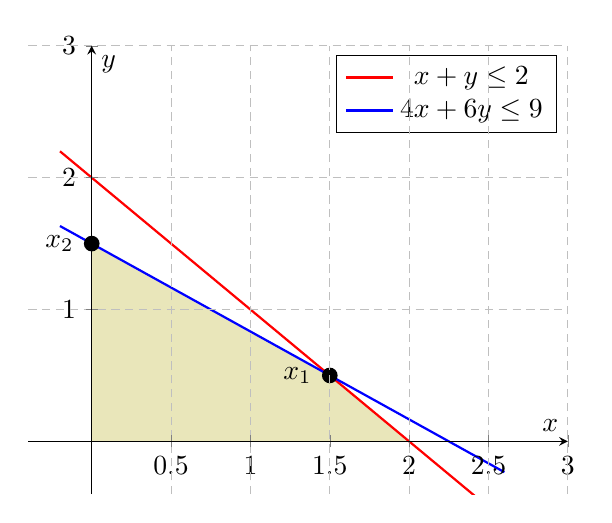
\begin{tikzpicture}
    \begin{axis}[
    grid,
    grid style={densely dashed},
    axis line style={->},
    axis lines=middle,
    xlabel=$x$,
    ylabel=$y$,
        xmin=-0.4, xmax=3,
        ymin=-0.4, ymax=3,
        axis lines=center,
       axis on top=true,
       domain=-0.2:2.6,
        ]
       \addplot [draw=red,thick,name path=A] {2-x}; \addlegendentry{$x + y \leq 2$}
       \addplot [draw=blue,thick,name path=B] {1.5-2/3*x}; \addlegendentry{$4x + 6y \leq 9$}
       \addplot [draw=none,name path=C] {0};
       \addplot[olive!20] fill between[of=B and C, soft clip={domain=0:1.5}];
       \addplot[olive!20] fill between[of=A and C, soft clip={domain=1.5:2}];
       \node[label={180:${x_{1}}$},circle,fill,inner sep=2pt] at (axis cs:1.5,0.5) {};
       \node[label={180:${x_{2}}$},circle,fill,inner sep=2pt] at (axis cs:0,1.5) {};
    \end{axis}
\end{tikzpicture}
\\ ب)
\begin{align*}
  x_{1} =
  \begin{bmatrix}
    \frac{3}{2} \\
    \frac{1}{2}
  \end{bmatrix} &&
  x_{2} =
  \begin{bmatrix}
    0 \\
    \frac{3}{2}
  \end{bmatrix}
\end{align*}
ج) چون هر نقطه روی پاره خط $x_{1}$ و $x_{2}$ جواب بهینه است، پس می‌توانیم چنین بنویسیم:
\begin{align*}
  A &= \{x \mid x = \lambda x_{1} + (1 - \lambda)x_{2};
  \quad 0 \leq \lambda \leq 1 \} \\
  \to A &= \{
      \begin{bmatrix}
        \frac{3}{2}\lambda \\
        \frac{3}{2} - \lambda
      \end{bmatrix}
  \mid \quad 0 \leq \lambda \leq 1 \}
\end{align*}


\subsection*{سؤال ۴۱}
الف) می‌دانیم اضافه کردن یک شرط جدید منتج به خط جدید در نمودار می‌شود. حال، این خط ممکن است ناحیه شدنی را قطع کند یا از آن عبور نکند. پس، ناحیه شدنی جدید کوچک‌تر مساوی ناحیه شدنی پیشین است. \\ \\
ب) چون با اضافه کردن شرط جدید، ناحیه شدنی به سمت بهینه بودن نخواهد رفت و تنها محدودتر خواهد شد، مقدار تابع هدف نیز کوچک‌تر نخواهد شد. پس مقدار تابع هدف جدید، بزرگ‌تر مساوی مقدار اصلی آن است.

\subsection*{سؤال ۴۲}
الف) اضافه کردن یک متغیر جدید باعث می‌شود تا یک بعد جدید در قسمت قیود بررسی شود. پس باعث می‌شود تا ناحیه شدنی بزرگ‌تر شود. \\ \\
ب) چون ناحیه شدنی افزایش می‌یابد، پس مقدار تابع هدف بزرگ‌تر نخواهد شد. پس مقدار تابع هدف جدید کوچک‌تر مساوی مقدار پیشین خواهد بود.

\subsection*{سؤال ۴۳}
الف) می‌دانیم حذف کردن یک شرط منتج به حذف یک خط در نمودار می‌شود. حال، این خط ممکن است در ابتدا باعث کوچک شدن ناحیه شدنی نشده باشد. پس ناحیه شدنی جدید بزرگ‌تر مساوی ناحیه شدنی پیشین است. \\ \\
ب) چون ناحیه شدنی می‌تواند افزایش یابد، پس مقدار تابع هدف بزرگ‌تر نخواهد شد. پس مقدار تابع هدف جدید کوچک‌تر مساوی مقدار پیشین خواهد بود.

\subsection*{سؤال ۴۴}
الف) حذف یک متغیر باعث می‌شود تا یک بعد را در قسمت قیود بررسی نکنیم. پس باعث می‌شود تا ناحیه شدنی کوچک‌تر شود. \\ \\
ب) چون ناحیه شدنی کاهش می‌یابد، پس مقدار تابع هدف کوچک‌تر نخواهد شد. پس مقدار تابع هدف جدید بزرگ‌تر مساوی مقدار پیشین خواهد بود.


\end{document}
